% OFDM description
\section{Description of OFDM} 
\indent OFDM stands for \textit{Orthogonal Frequency Division Multiplexing}. It relies on different principles used together to combine advantages.\\
%
\begin{figure}[H]
  \centering
  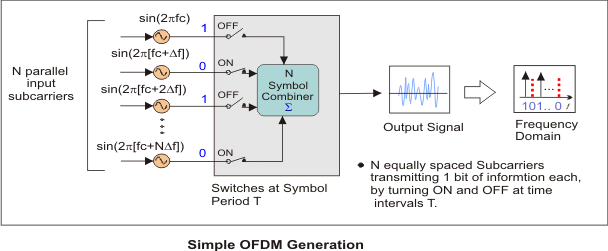
\includegraphics[width=\textwidth]{figures/ofdm-simplegenerator.png}
  \caption{Modulation of signals using OFDM technique \textbf{[source: Keysight]}}
  \label{fig:OFDMGenerator}
\end{figure}
%% TODO : Remove image integrated caption !!
\indent The most basic of these principles is the FDM (\textit{Frequency Division Multiplexing}). It consists in modulating several ($N$) signals using a QAM (\textit{Quadrature Amplitude Modulation}) scheme, with sub-carriers that are regularly spaced by $\Delta f$, see \figref{fig:OFDMGenerator}.
All these modulated signals are then put into an IFFT (\textit{Inverse Fast Fourier Transform}) and summed into a single signal, updated periodicly according to the symbol period $T$ and sent through the desired medium. At the receiver end, the inverse procedure is applied.\\
%
\indent The second main concept is the orthogonality of the sub-carriers. When passing to the frequency domain, each sub-carrier will result in a sinc function. Therefore, the spacing, $\Delta f$, between each of them is chosen so that, in frequency domain, each sub-carrier overlap the others orthogonally, which means all the sinc functions have zero crossing and their side-loops cancel each other, while peaks remain distinguishable, see \figref{fig:freqOrthoSinc}.
%
\begin{figure}[H]
  \centering
  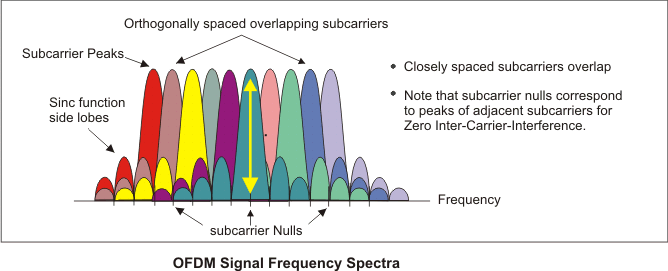
\includegraphics[width=\textwidth]{figures/ofdm-orthogonalspacedsubcarriers.png}
  \caption{Frequency spectrum of OFDM signal \textbf{[source: Keysight]}}
  \label{fig:freqOrthoSinc}
\end{figure}
%
Since, there is no undesirable interference due to frequency overlapping, the spacing between each sub-carrier can be very short. To maintain the orthogonality, this spacing, $\Delta f$, actually has to be the inverse of a symbol period, $T$ :
\begin{flalign}
\eq{\Delta f}{1/T}
\end{flalign}\\
\indent Coming from this relation, and by sending information on parallel channels, it is possible to increase the overall data rate and therefore, the spectral efficiency, while decreasing the data rate on each subchannel. This helps to reduce potential inter-symbol interferences (ISI) at the receiver end, that could happen due to wave reflection, refraction or other multi-path phenomena \cite{RadioElOFDM} and is reinforced by a guard interval between each symbol.\\
%
\indent However, one of the worst disadvantages of OFDM is the high peak-to-power ratio which makes the use of this technique inefficient in terms of energy for small and portable devices.